\documentclass[a4paper,12pt]{article}
\usepackage[utf8]{inputenc}
\usepackage[spanish]{babel}
\usepackage{graphicx}
\usepackage{url}
\usepackage{float}
\usepackage{listings}
\usepackage{xcolor}

\definecolor{gris}{RGB}{123, 126, 132}
\definecolor{morado}{RGB}{157, 101, 255}
\definecolor{amarillo}{RGB}{253,151,31}
\definecolor{magenta}{RGB}{249,38,114}

\lstdefinestyle{customJava}{
    frame=tb,
    language=Java,
    basicstyle=\footnotesize\ttfamily,
    backgroundcolor=\color{white},   
    commentstyle=\itshape\color{gris},
    keywordstyle=\bfseries\color{magenta},
    numberstyle=\color{morado},
    stringstyle=\color{amarillo},
    identifierstyle=\color{magenta},
    basicstyle=\footnotesize,
    breakatwhitespace=false,         
    breaklines=true,                 
    captionpos=b,
    keepspaces=true,                 
    numbers=left,                    
    numbersep=5pt,                  
    showspaces=false,                
    showstringspaces=false,
    showtabs=false,                  
    tabsize=2,
    morekeywords={web-app, encoding, xmlns, xmlns:xsi, xsi:schemaLocation}
}

%opening
\title{Tarea No. 7. Data Access Object}
\author{Barrera Pérez Carlos Tonatihu \\ Profesor: José Asunción Enríquez 
Zárate 
\\ Web Application Development \\ Grupo: 3CM9 }

\begin{document}

\maketitle
\newpage
\tableofcontents
\newpage

\section{Introducción}
Si  las aplicaciones usan diferentes tipos de almacenamientos persistentes 
(bases de datos relacionales, bases de datos orientadas a objetos, ficheros 
planos, etc.), existe aún más diversidad entre las distintas APIs que se 
necesitan y sus características.

Al codificar las llamadas a estos APIs, desde los componentes una aplicación, se 
creará una dependencia directa entre el código de los componentes de la 
aplicación y el código de acceso a los datos. Este acoplamiento, haría difícil y 
tedioso migrar la aplicación de un tipo de fuente de datos a otro, e implicaría 
cambiar los componentes para modificar el acceso a los datos.
Utilizar un Data Access Object (DAO) para abstraer y encapsular todos los 
accesos a la fuente de datos. El DAO maneja la conexión con la fuente de datos 
para obtener y almacenar datos \cite{oracle}. 

\section{Desarrollo}
El DAO implementa el mecanismo de acceso requerido para trabajar con la fuente 
de datos. Esta fuente de datos puede ser un almacenamiento persistente como una 
RDMBS, un servicio externo como un intercambio B2B, un repositorio LDAP, o un 
servicio de negocios al que se accede mediante CORBA Internet Inter-ORB Protocol 
(IIOP) o sockets de bajo nivel. Los componentes de negocio que tratan con el DAO 
utilizan un interface simple expuesto por el DAO para sus clientes. El DAO 
oculta completamente los detalles de implementación de la fuente de datos a sus 
clientes. Como el interface expuesto por el DAO no cambia cuando cambia la 
implementación de la fuente de datos subyacente, este patrón permite al DAO 
adaptarse a diferentes esquemas de almacenamiento sin que esto afecte a sus 
clientes o componentes de negocio. Esencialmente, el DAO actúa como un adaptador 
entre el componente y la fuente de datos \cite{geek}.

La estructura y sus componentes de esta arquitectura son las siguiente:

\begin{figure}[H]
\begin{center}
 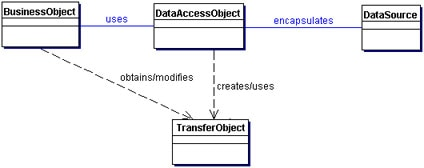
\includegraphics[width=13cm]{clases.jpg}
 % estructura.png: 800x436 px, 96dpi, 21.16x11.53 cm, bb=0 0 600 327
 \caption{Estructura básica \cite{oracle}}
 \label{fig:control}
\end{center}
\end{figure}

\begin{itemize}
  \item BusinessObject: Representa los datos del cliente. Es el objeto que 
requiere el acceso a la fuente de datos para obtener y almacenar datos. 
Podríamos implementar un BusinessObject como un bean de sesión, un bean de 
entidad o cualquier otro objeto Java, además de como un Servlet o como un bean 
de apoyo.
  \item DataAccessObject: Es el objeto principal de este patrón. El 
DataAccessObject abstrae la implementación del acceso a datos subyacente al 
BusinessObject para permitirle un acceso transparente a la fuente de datos. El 
BusinessObject también delega las operaciones de carga y almacenamiento en el 
DataAccessObject.
  \item DataSource: Representa la implementación de la fuente de datos. Una 
fuente de datos podría ser una base de datos como un RDBMS, un OODBMS, un 
repositorio XML, un fichero plano, etc. También lo pueden ser otros sitemas 
(mainframes/legales), servicios (servicio B2B u oficina de tarjetas de 
crédito), o algún tipo de repositorio (LDAP).
  \item TransferObject: Representa un TransferObject utilizado para el 
transporte de datos. DataAccessObject podría utilizar un TransferObject para 
devolver los datos al cliente. El DataAccessObject también podría recibir datos 
desde el cliente en un TransferObject para actualizar los datos en la fuente de 
datos.
\end{itemize}

\begin{figure}[H]
\begin{center}
 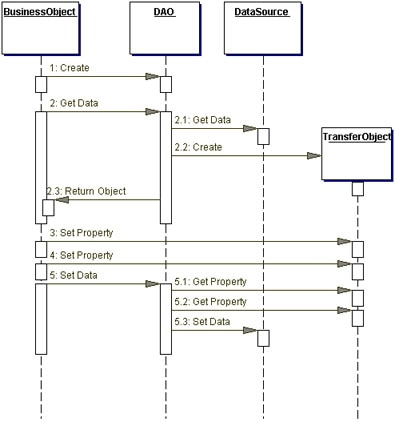
\includegraphics[width=13cm]{interaccion.jpg}
 % estructura.png: 800x436 px, 96dpi, 21.16x11.53 cm, bb=0 0 600 327
 \caption{Interacción entre todos los componentes \cite{oracle}}
 \label{fig:interaccion}
\end{center}
\end{figure}

\section{Conclusiones}
El trabajar utilizando DAOs nos proporciono grandes ventajas ya que nos permite 
una mejor separacion entre distintas partes de la aplicación por lo que les 
proporiona indepencia y facilidad de manipular, de esta forma al tener una capa 
DAO hace la tarea de cambiar de palataforma de persistencia algo facil.

Sin embargo es importante considerar en que situaciones el implementar este 
patrón nos proporcionará los resultados esperados ya que se debe de saber como 
aplicarlo, de lo contrario podría provocar que se duplique el código y una 
falta de abstracción, lo cual solo ocasionara más problemas de los que podria 
haber solucionado.


\bibliographystyle{ieeetr}
\bibliography{referencias}

\end{document}
